\documentclass[11pt, oneside]{article}   	% use "amsart" instead of "article" for AMSLaTeX format
\usepackage{geometry}                		% See geometry.pdf to learn the layout options. There are lots.
\geometry{letterpaper, margin=.5in}                   		% ... or a4paper or a5paper or ... 
%\geometry{landscape}                		% Activate for rotated page geometry
%\usepackage[parfill]{parskip}    		% Activate to begin paragraphs with an empty line rather than an indent
\usepackage{graphicx}				% Use pdf, png, jpg, or eps§ with pdflatex; use eps in DVI mode
								% TeX will automatically convert eps --> pdf in pdflatex		
\usepackage{wrapfig}								
\usepackage{amssymb}
%SetFonts
%SetFonts
\date{}							% Activate to display a given date or no date

\begin{document}

\section*{Part A}
\begin{wrapfigure}[16]{r}{0.5\textwidth}
\begin{flushright}
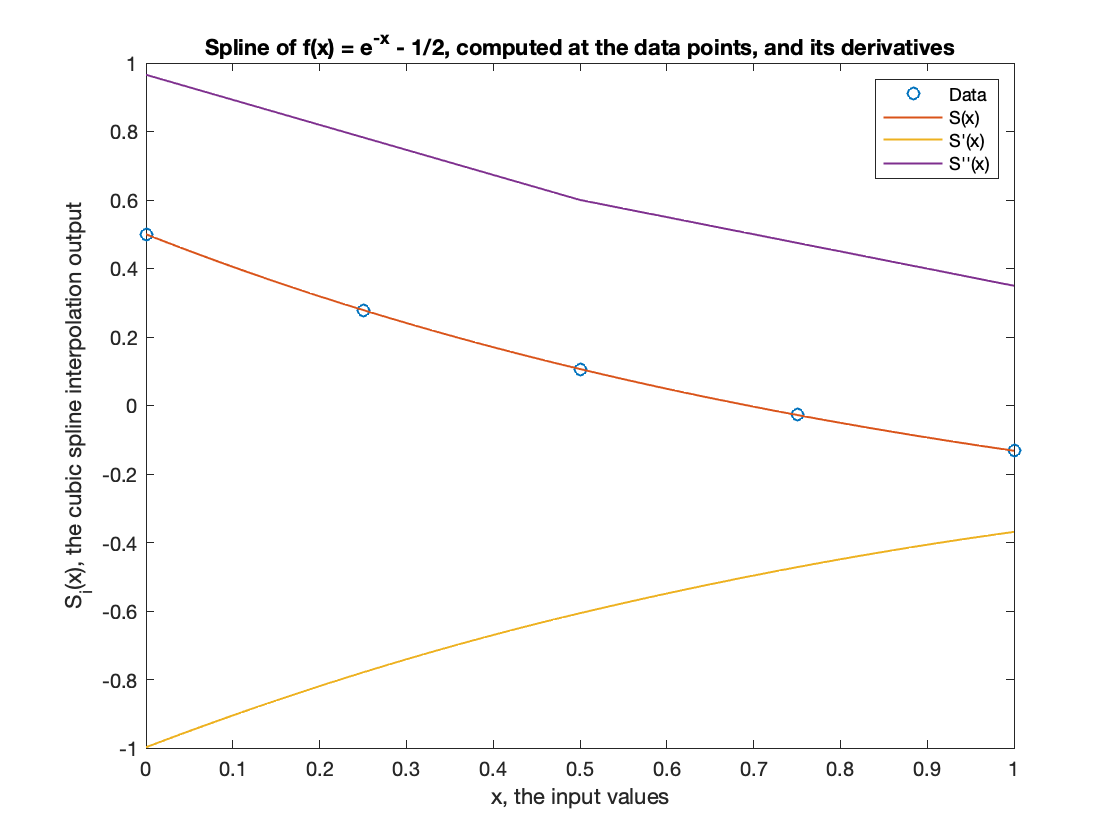
\includegraphics [scale=.25] {PartA.png}
\end{flushright}
\end{wrapfigure}

The function $f(x) = e^{-x} - \frac{1}{2}$, evaluated at $x = 0, 0.25, 0.5, 0.75, 1$, is given by the circular data points in the graphic. From these data points, a cubic spline with not-a-knot end conditions was constructed, and its first and second derivatives were computed. Each is shown, with their values graphed in intervals of 1/100th.\\

Since the spline is cubic, it takes on the form $f_i(x) = a_i + b_ix + c_ix^2 + d_ix^3$. The coefficients for the spline $f$ are as follows: \\

$~$\\
$   -0.1218  ~~  0.4828 ~~  -0.9979 ~~ 0.5000$\\
$   -0.1218  ~~ 0.3914 ~~  -0.7793  ~~  0.2788$\\
$   -0.0835  ~~  0.3001 ~~  -0.6065  ~~  0.1065$\\
$   -0.0835  ~~  0.2374 ~~  -0.4721 ~~  -0.0276$\\

From which the derivatives are simple to construct. The approximations for $f'(0.5)$ and $f''(0.5$ are $s'(0.5) \approx -0.6065$, $s''(0.5) \approx 0.6001$, and their absolute errors are given by $|s'(0.5) - f'(0.5)| \approx 7.9565e^{0.5}$ and $|s''(0.5) - f''(0.5)| \approx 0.0064$.

\section*{Part B}



\end{document}  